\documentclass[a4paper, 12pt]{article}
% math symbols
\usepackage{amssymb}
\usepackage{amsmath}
\usepackage{mathrsfs}
\usepackage{physsummer}


\usepackage{enumitem}
\usepackage[margin = 2cm]{geometry}

\tolerance = 1000
\emergencystretch = 0.74cm



\pagestyle{empty}
\parindent = 0mm

\setphysstyle{ФМЛ 239, 9 класс}{Занятие 7 \\ подготовка к районному
  туру}{14 ноября 2015}

\begin{document}

\Large

\taskpic{ Из дырки в стене во все стороны по полу начинают
  одновременно разбегаться муравьи. Скорость всех муравьев одинакова и
  равна $v$. Пылесос со щеткой, расположенной под углом
  $\alpha=45^{\circ}$ к стенке, движется вдоль стены со скоростью $u$
  так, как показано на рисунке. Через какое время $t$ первый муравей
  попал под щетку, если начальное расстояние между точкой $A$ щетки и
  дыркой в стене равно $l$?  } {
  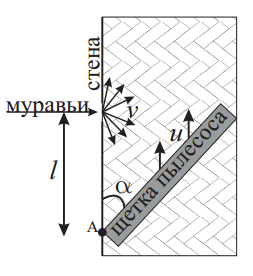
\includegraphics[width=4cm]{2015_11_14_239_7_1.png}
}
% Район-2015-9

\task{ В морозильной камере, потребляющей из сети мощность
  $P=100 \mbox{ Вт}$, находится $m=20 \mbox{ кг}$ воды при температуре
  $T=0^{\circ}\mbox{C}$. Вся вода замерзает за $t=1$ сутки. Какое
  количество теплоты выделяется за это время в окружающую среду?
  Считайте, что конечная температура льда
  $0^{\circ}\mbox{C}$. Удельная теплота плавления льда $\lambda = 330
  \mbox{ кДж/кг}$.}
% Район-2007-9

\taskpic{ На секундомер с металлическим ободом и металлической
  стрелкой подали постоянное напряжение: к началу стрелки и к точке
  <<45 секунд>> на ободе. Также в схему последовательно включили
  лампочку. Через сколько секунд после запуска яркость лампочки будет
  минимальной? Через сколько — максимальной? }
{
  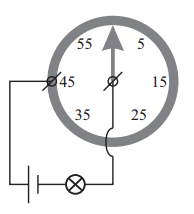
\includegraphics[width=4cm]{2015_11_14_239_7_3.png}
}
% Район-2015-9

\end{document}


%%% Local Variables: 
%%% mode: latex
%%% TeX-engine:xetex
%%% TeX-PDF-mode: t
%%% End:
